\documentclass{article}
\usepackage{hyperref}
\usepackage{amsmath}
\usepackage{amssymb}
\usepackage{pgfplots}
\usepackage{float}
\usepackage{tikz}
\usepackage{todonotes}
\usepackage[shortlabels]{enumitem}
\usepackage{algorithm}
\usepackage{algpseudocode}
\usepackage{graphicx}
\usepackage{subcaption}

% For InkScape tex files:
\usepackage[pdf]{pstricks}

\renewcommand{\Re}{\mathbb{R}}
\newcommand{\Li}{\mathcal{L}}
\newcommand{\Ex}{\mathbb{E}}
\renewcommand{\Pr}{\mathbb{P}}
\newcommand{\Hy}{\mathcal{H}}
\newcommand{\sign}{\text{sign}}
\newcommand{\error}{\text{error}}
\newcommand{\dist}{\text{dist}}
\newcommand{\given}{\middle\vert}
\newcommand{\LCA}{\text{LCA}}

\newcommand\bigO[1]{
    \ensuremath{\mathcal{O}\left(#1\right)}
    }

\newcommand{\sigmoidPlot}{
    
    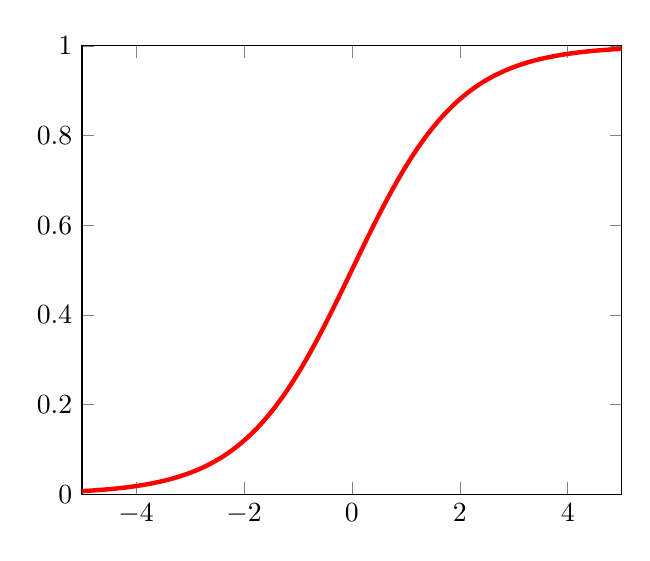
\begin{tikzpicture}
        \begin{axis}[xmin=-5, xmax=5, ymin=0, ymax=1, samples=150]
        \addplot[red, ultra thick] {1/(1+exp(-x))};
        \end{axis}
    \end{tikzpicture}
    
    }

\usetikzlibrary{positioning, calc}
\usetikzlibrary{arrows.meta}

\tikzstyle{circlebox}=[circle,thick,draw=black!75,minimum size=8mm]
\tikzstyle{smallcirclebox}=[circle,thick,draw=black!75,fill=black!75,minimum 
size=4mm]
\tikzstyle{inputnode}=[circlebox, draw=blue!75]
\tikzstyle{hiddennode}=[circlebox, draw=orange!75]
\tikzstyle{outputnode}=[circlebox, draw=orange!75]
\tikzstyle{simplebox}=[rectangle,thick,draw=black!75,
fill=black!20,minimum size=4mm]
\tikzstyle{textbox}=[rectangle,thick,minimum size=4mm,draw=black!0,
fill=black!0]
\tikzstyle{halfvdistance}=[yshift=-0.7cm]
\tikzstyle{abovebetween}=[xshift=-2.7mm]
\tikzstyle{edgepath} = [-Latex,->,shorten >=1pt,-stealth,semithick, rounded 
corners=5pt]

\def \nodedv {0.735cm}
\def \nodedh {0.65cm}

\tikzset{
    between/.style args={#1 and #2}{
        at = ($(#1)!0.5!(#2)$)
    }
}
\usepackage{xinttools} % for the \xintFor***

\def\biglen{20cm} % playing role of infinity (should be < .25\maxdimen)
% define the "half plane" to be clipped (#1 = half the distance between cells)
\tikzset{
    half plane/.style={ to path={
            ($(\tikztostart)!.5!(\tikztotarget)!#1!(\tikztotarget)!\biglen!90:(\tikztotarget)$)
            -- 
            ($(\tikztostart)!.5!(\tikztotarget)!#1!(\tikztotarget)!\biglen!-90:(\tikztotarget)$)
            -- ([turn]0,2*\biglen) -- ([turn]0,2*\biglen) -- cycle}},
    half plane/.default={1pt}
}

\def\n{23} % number of random points
\def\maxxy{4} % random points are in [-\maxxy,\maxxy]x[-\maxxy,\maxxy]

\newcommand{\voronoi}[2]{
    \def \n{#1}
    \def \maxxy{#2}
    \begin{tikzpicture}
    % generate random points
    \pgfmathsetseed{1908} % init random with the year Voronoi published his 
    %paper ;)
    \def\pts{}
    \xintFor* ##1 in {\xintSeq {1}{\n}} \do{
        \pgfmathsetmacro{\ptx}{.9*\maxxy*rand} % random x in 
        %[-.9\maxxy,.9\maxxy]
        \pgfmathsetmacro{\pty}{.9*\maxxy*rand} % random y in 
        %[-.9\maxxy,.9\maxxy]
        \edef\pts{\pts, (\ptx,\pty)} % stock the random point
    }
    
    % draw the points and their cells
    \xintForpair ##1##2 in \pts \do{
        \edef\pta{##1,##2}
        \begin{scope}
        \xintForpair ##3##4 in \pts \do{
            \edef\ptb{##3,##4}
            \ifx\pta\ptb\relax % check if (#1,#2) == (#3,#4) ?
            \tikzstyle{myclip}=[];
            \else
            \tikzstyle{myclip}=[clip];
            \fi;
            \path[myclip] (##3,##4) to[half plane] (##1,##2);
        }
        \clip (-\maxxy,-\maxxy) rectangle (\maxxy,\maxxy); % last clip
        \pgfmathsetmacro{\randhue}{rnd}
        \definecolor{randcolor}{hsb}{\randhue,.5,1}
        \fill[randcolor] (##1,##2) circle (4*\biglen); % fill the cell with 
        %random color
        \fill[draw=red,very thick] (##1,##2) circle (1.4pt); % and draw the 
        %point
        \end{scope}
    }
    \pgfresetboundingbox
    \draw (-\maxxy,-\maxxy) rectangle (\maxxy,\maxxy);
    \end{tikzpicture}
}